\documentclass{beamer}
\usepackage[utf8]{inputenc}

\usetheme{Madrid}
\usecolortheme{default}
\usepackage{amsmath,amssymb,amsfonts,amsthm}
\usepackage{txfonts}
\usepackage{tkz-euclide}
\usepackage{listings}
\usepackage{adjustbox}
\usepackage{array}
\usepackage{tabularx}
\usepackage{gvv}
\usepackage{lmodern}
\usepackage{circuitikz}
\usepackage{tikz}
\usepackage[utf8]{inputenc}

\usetheme{Madrid}
\usecolortheme{default}
\usepackage{amsmath,amssymb,amsfonts,amsthm}
\usepackage{txfonts}
\usepackage{tkz-euclide}
\usepackage{listings}
\usepackage{adjustbox}
\usepackage{array}
\usepackage{tabularx}
\usepackage{gvv}
\usepackage{lmodern}
\usepackage{circuitikz}
\usepackage{tikz}
\usepackage{graphicx}

\setbeamertemplate{page number in head/foot}[totalframenumber]

\usepackage{tcolorbox}
\tcbuselibrary{minted,breakable,xparse,skins}



\definecolor{bg}{gray}{0.95}
\DeclareTCBListing{mintedbox}{O{}m!O{}}{%
  breakable=true,
  listing engine=minted,
  listing only,
  minted language=#2,
  minted style=default,
  minted options={%
    linenos,
    gobble=0,
    breaklines=true,
    breakafter=,,
    fontsize=\small,
    numbersep=8pt,
    #1},
  boxsep=0pt,
  left skip=0pt,
  right skip=0pt,
  left=25pt,
  right=0pt,
  top=3pt,
  bottom=3pt,
  arc=5pt,
  leftrule=0pt,
  rightrule=0pt,
  bottomrule=2pt,

  colback=bg,
  colframe=orange!70,
  enhanced,
  overlay={%
    \begin{tcbclipinterior}
    \fill[orange!20!white] (frame.south west) rectangle ([xshift=20pt]frame.north west);
    \end{tcbclipinterior}},
  #3,
}
\lstset{
    language=C,
    basicstyle=\ttfamily\small,
    keywordstyle=\color{blue},
    stringstyle=\color{orange},
    commentstyle=\color{green!60!black},
    numbers=left,
    numberstyle=\tiny\color{gray},
    breaklines=true,
    showstringspaces=false,
}
%------------------------------------------------------------
%This block of code defines the information to appear in the
%Title page
\title %optional
{4.13.19}
\date{October  2025}
%\subtitle{A short story}

\author % (optional)
{Bhoomika L - EE25BTECH11014}

\begin{document}


\frame{\titlepage}
\begin{frame}{Question} If the line $2x + y = k$ passes through the point which divides the line segment joining the points $\bark{1, 1}$ and $\brak{2, 4}$ in the ratio $3:2$, then $k$ equals
\begin{multicols}
\begin{enumerate}
    \item $\frac{29}{5}$
    \item $5$
    \item $6$
    \item $\frac{11}{5}$
\end{enumerate}
\end{multicols}
\end{frame}

\begin{frame}{Solution}
Let the point $\vec{C}$ divide the line segment joining $\vec{A}$ and $\vec{B}$ in the ratio $3:2$ where
\begin{align}
     \vec{A}=\myvec{1\\1}\\
    \vec{B}=\myvec{2\\4}\\
\end{align}
\end{frame}

\begin{frame}{Formula}
	By section formula,
\begin{align}
   \vec{C}=\frac{\lambda\vec{B}+\vec{A}} {\brak{\lambda +1}}.\\  
    Here \brak{\lambda=\frac{3}{2}}
\end{align}

The equation of the line can be represented as:
\begin{align}
    \vec{n^T}\vec{x}=c_1\\
 where  \ \vec{n^T}=\myvec{2&1} \ and \ c_1=k.
\end{align}
\end{frame}

\begin{frame}{Solution}

As $\vec{C}$ lies on the above line,
\begin{align}
  \vec{n^T}\vec{C}=c_1\\
 \myvec{2&1}\frac{\lambda\vec{B}+\vec{A}} {\brak{\lambda +1}}=k\\
 \frac{1}{5}\myvec{2&1}\brak{3\vec{B}+2\vec{A}}=k\\
 \frac{1}{5}\myvec{2&1}\brak{\myvec{6\\12}+\myvec{2\\2}}=k\\
 \frac{1}{5}\myvec{2&1}\myvec{8\\14}=k\\
 k=\frac{16}{5}+\frac{14}{5}=6.
 \end{align}
\end{frame}

\begin{frame}{Plot}
    \centering
    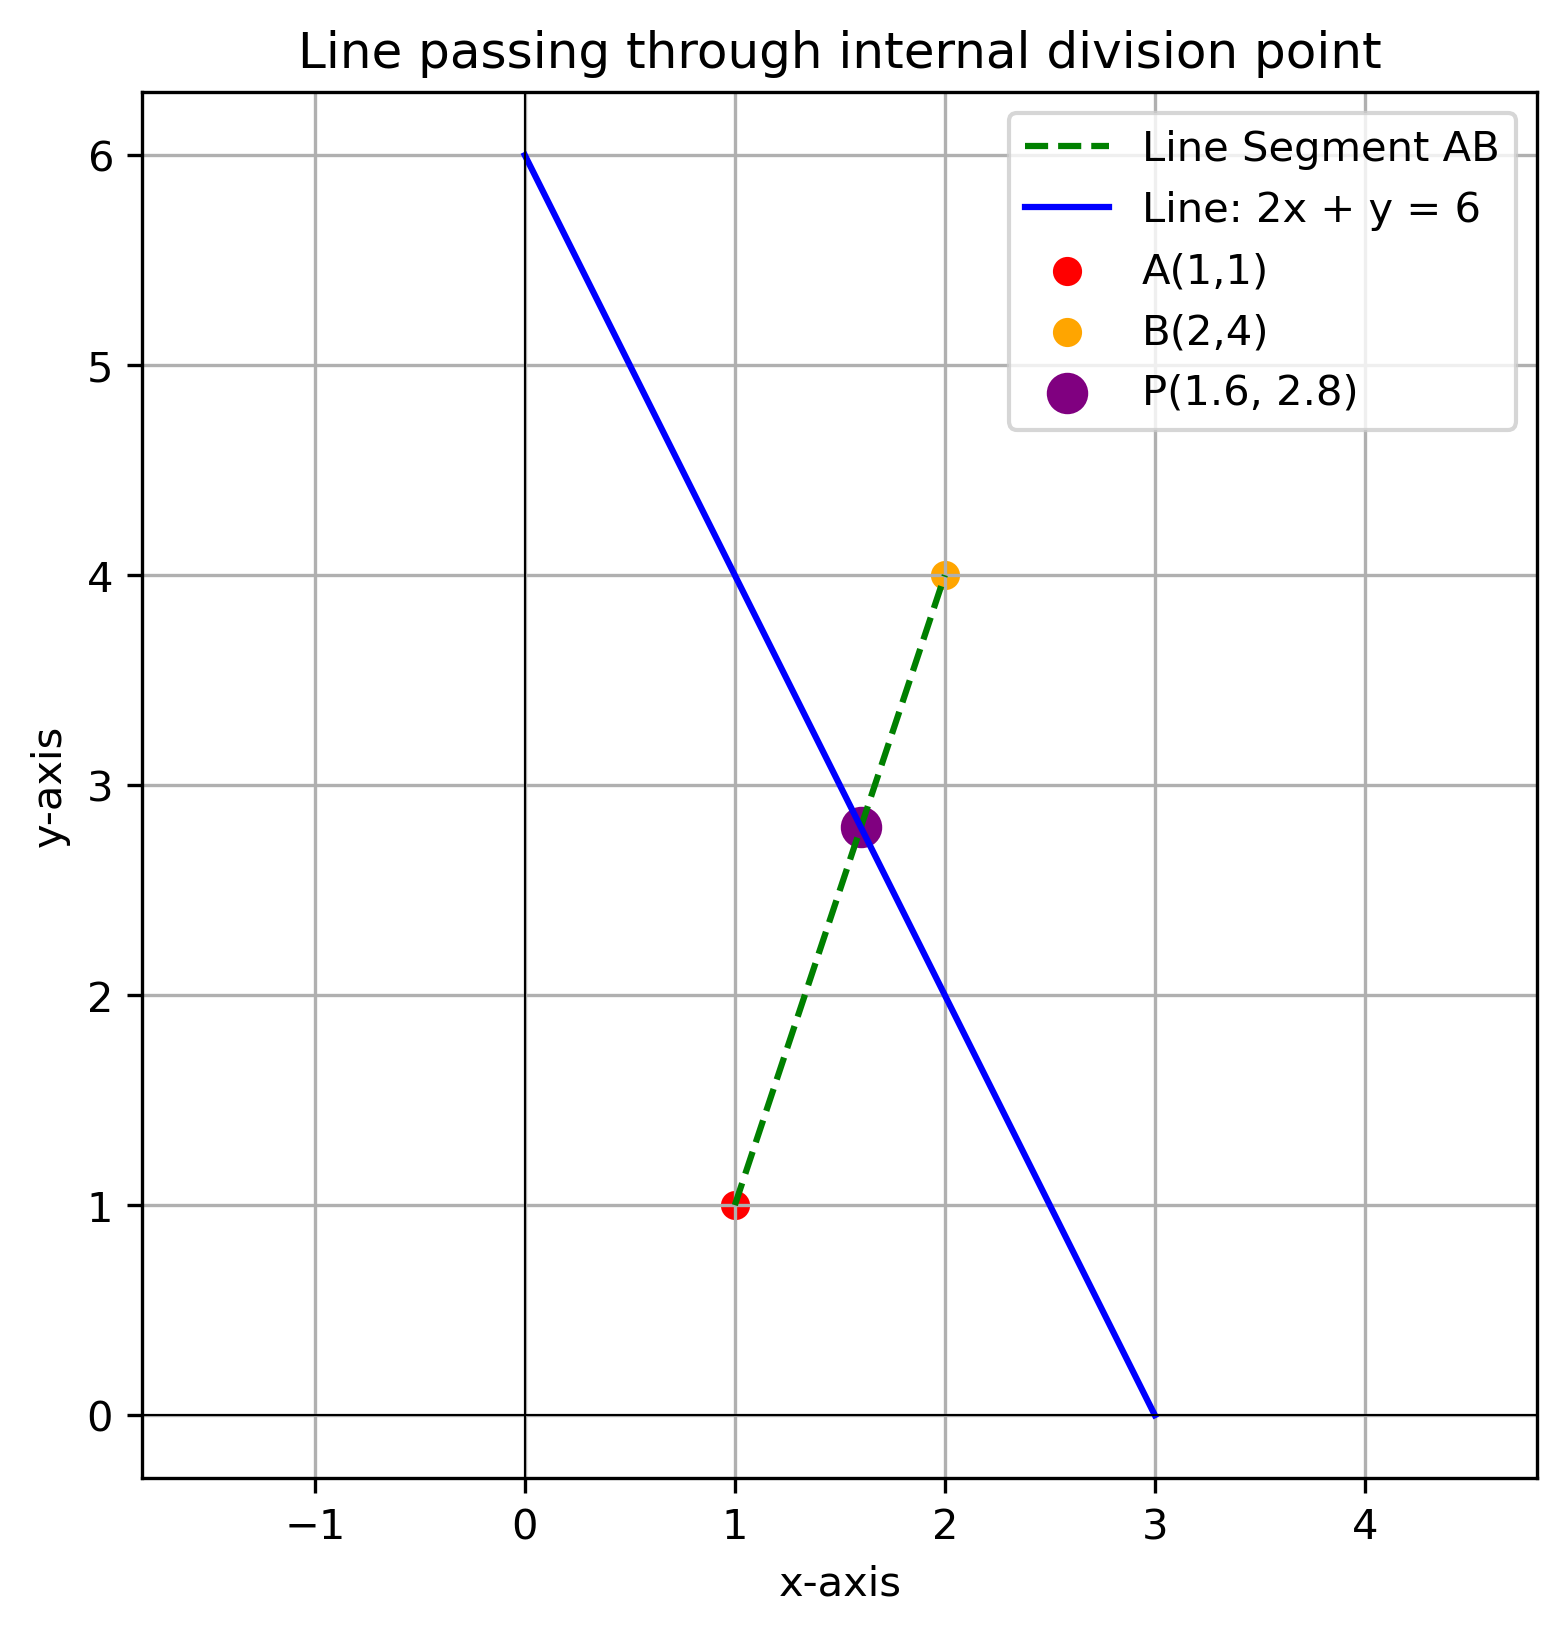
\includegraphics[width=\columnwidth, height=0.8\textheight, keepaspectratio]{../Figs/findk.png}     
\end{frame}

 \begin{frame}[fragile]
\frametitle{C Code }
\begin{lstlisting}
#include <stdio.h>
// sol[0] = x, sol[1] = y, sol[2] = k
void find_k(double sol[3]) {
   
    double x1 = 1, y1 = 1;
    double x2 = 2, y2 = 4;
    int m = 3, n = 2;

    // Internal division point (x, y)
    double x = (m*x2 + n*x1) / (double)(m+n);
    double y = (m*y2 + n*y1) / (double)(m+n);

    double k = 2*x + y;

    // Store results
    sol[0] = x;
    sol[1] = y;
    sol[2] = k;
}
\end{lstlisting}
\end{frame}

 \begin{frame}[fragile]
\frametitle{Python Code }
\begin{lstlisting}
import ctypes
import numpy as np
import matplotlib.pyplot as plt

#  Call C library
lib = ctypes.CDLL("./findk.so")

# Define argument types
lib.find_k.argtypes = [ctypes.POINTER(ctypes.c_double)]

# Prepare result array
sol = (ctypes.c_double * 3)()

\end{lstlisting}
\end{frame}

 \begin{frame}[fragile]
\frametitle{Python Code }
\begin{lstlisting}
# Call C function
lib.find_k(sol)

# Extract results
x, y, k = sol[0], sol[1], sol[2]

print(f"Point dividing AB in 3:2 = ({x}, {y})")
print(f"Value of k = {k}")

#  Plot the graph
# Given points
A = np.array([1, 1])
B = np.array([2, 4])
P = np.array([x, y])   # Use point from C code
\end{lstlisting}
\end{frame}

 \begin{frame}[fragile]
\frametitle{Python Code }
\begin{lstlisting}
# Line equation: 2x + y = k  => y = k - 2x
x_vals = np.linspace(0, 3, 100)
y_vals = k - 2*x_vals

plt.figure(figsize=(6,6))

# Plot line segment AB
plt.plot([A[0], B[0]], [A[1], B[1]], 'g--', label='Line Segment AB')

# Plot line 2x+y=k
plt.plot(x_vals, y_vals, 'b', label=f'Line: 2x + y = {k:.0f}')

# Plot points
plt.scatter(*A, color='red', label='A(1,1)')
plt.scatter(*B, color='orange', label='B(2,4)')
plt.scatter(*P, color='purple', s=80, marker='o', label=f'P({x:.1f},{y:.1f})')
\end{lstlisting}
\end{frame}

 \begin{frame}[fragile]
\frametitle{Python Code }
\begin{lstlisting}
# Labels
plt.xlabel('x-axis')
plt.ylabel('y-axis')
plt.title('Line passing through internal division point')
plt.axhline(0, color='black', linewidth=0.5)
plt.axvline(0, color='black', linewidth=0.5)
plt.legend()
plt.grid(True)
plt.axis("equal")

# Save the figure
plt.savefig("findk.png", dpi=300, bbox_inches='tight')
plt.show()
\end{lstlisting}
\end{frame}

\end{document}
